\begin{itemize}
	\item Решая численно линейное уравнение эволюции, мы получаем в момент $T_{\odot}$ конечное распределение, откуда находится темп аннигилляции, что эквивалентно решению с нелинейной добавкой от аннигиляции.
\end{itemize}


\begin{figure}[!h]
	\centering
	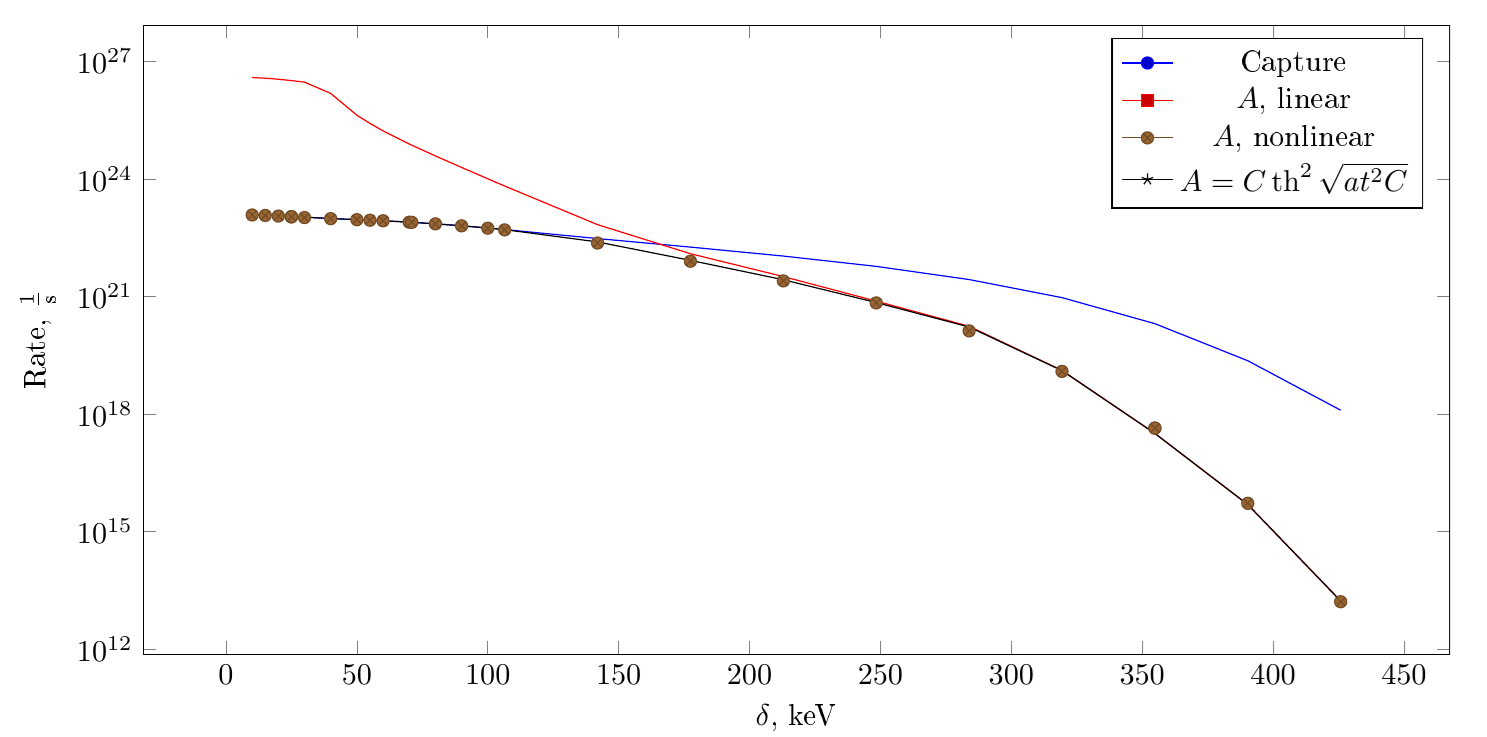
\includegraphics[width=0.7\textwidth]{images/LinearNonLinear.png}
	\caption{Зависимость от $\delta$ захвата и аннигиляции при линейной и нелинейной эволюции для $m_{\chi} = 100\text{GeV}$}
\end{figure}
